% Week 4: Convolutional Neural Networks I
\chapter{Week 4: Convolutional Neural Networks I}
\label{ch:week4}

\begin{quickref}[Chapter Overview]
\textbf{Core goal:} Understand how convolutional neural networks exploit spatial structure for efficient image processing.

\textbf{Key topics:}
\begin{itemize}
    \item Why CNNs? Challenges with fully connected layers for images
    \item Convolution and cross-correlation operations
    \item Padding strategies and output dimensions
    \item Pooling for dimensionality reduction and translation invariance
    \item Multi-channel inputs and outputs
    \item CNN architectures (LeNet) and feature visualisation
\end{itemize}

\textbf{Key equations:}
\begin{itemize}
    \item Cross-correlation: $(X * W)_{ij} = \sum_{p,q} x_{i+p, j+q} \cdot w_{p,q}$
    \item Max pooling: $h^{[l]}_{jk} = \max_{p,q} h^{[l-1]}_{j \cdot s + p, k \cdot s + q}$
    \item Output size: $\lfloor (d + 2P - r) / S \rfloor + 1$
\end{itemize}
\end{quickref}

%==============================================================================
\section{Computer Vision Tasks}
%==============================================================================

Computer vision encompasses a broad range of tasks that require machines to interpret visual information. The fundamental tasks include:

\begin{itemize}
    \item \textbf{Image classification}: Assigning a label to an entire image (e.g., ``cat'', ``dog'')
    \item \textbf{Object detection}: Locating and classifying multiple objects within an image
    \item \textbf{Semantic segmentation}: Classifying each pixel into a category
    \item \textbf{Instance segmentation}: Distinguishing individual objects of the same class
\end{itemize}

\begin{figure}[H]
    \centering
    \includegraphics[width=1\linewidth]{images/week_4/Screenshot 2024-10-22 at 17.49.34.png}
    \caption{Common computer vision tasks: classification assigns one label to the whole image; detection locates objects with bounding boxes; segmentation classifies every pixel.}
    \label{fig:cv-tasks}
\end{figure}

\subsection{Human vs Computer Perception}

Humans and computers process visual information in fundamentally different ways. Understanding this difference motivates why specialised architectures like CNNs are necessary.

\begin{quickref}[Human vs Machine Vision]
\textbf{Humans:}
\begin{itemize}
    \item Look for local features (edges, textures, shapes)
    \item Automatically ignore irrelevant information
    \item Recognise objects regardless of position, scale, or lighting
    \item Process visual information hierarchically (low-level to high-level)
\end{itemize}

\textbf{Computers:}
\begin{itemize}
    \item See a matrix of pixel values (typically 0--255 for 8-bit images)
    \item Colour images have multiple channels (RGB = 3 channels)
    \item Can also process hyperspectral images (100s of channels)
    \item Require explicit algorithms to extract meaning from raw pixels
\end{itemize}
\end{quickref}

The challenge for computer vision is to bridge this gap: to design algorithms that can extract meaningful, high-level understanding from raw numerical pixel values, much as humans effortlessly do.

%==============================================================================
\section{Why Convolutional Layers?}
%==============================================================================

Before CNNs became dominant, image processing with neural networks used fully connected layers. This approach has severe limitations that convolutional layers elegantly solve.

\begin{quickref}[CNN Motivation]
CNNs address three key challenges:
\begin{enumerate}
    \item \textbf{Reduce parameters}: Weight sharing across spatial locations
    \item \textbf{Leverage locality}: Nearby pixels are more related than distant ones
    \item \textbf{Translation invariance}: Detect features regardless of position
\end{enumerate}
\end{quickref}

\subsection{Challenge 1: Spatial Structure}

Fully connected layers treat every input independently, destroying the spatial relationships that are crucial for understanding images.

\begin{figure}[H]
    \centering
    \includegraphics[width=0.5\linewidth]{images/week_4/fully connected.png}
    \caption{Fully connected network: every neuron connects to every input. For images, this means flattening the 2D structure into a 1D vector.}
    \label{fig:fully-connected}
\end{figure}

\begin{rigour}[Fully Connected Layer]
In a fully connected layer, each neuron computes a weighted sum of \emph{all} inputs:
\[
h^{[l]}_j = \sigma \left( \sum_{i=1}^{H^{[l-1]}} W^{[l]}_{ij} h^{[l-1]}_i + b^{[l]}_j \right)
\]

where:
\begin{itemize}
    \item $h^{[l-1]}_i$ is the activation of neuron $i$ in the previous layer $(l-1)$
    \item $W^{[l]}_{ij}$ is the weight connecting neuron $i$ in layer $l-1$ to neuron $j$ in layer $l$
    \item $b^{[l]}_j$ is the bias term for neuron $j$ in layer $l$
    \item $\sigma(\cdot)$ is the activation function (ReLU, sigmoid, etc.)
    \item The summation runs over all $H^{[l-1]}$ neurons in the previous layer
\end{itemize}

\textbf{Problem for images:}
\begin{itemize}
    \item Images must be \textbf{flattened} to a 1D vector before input
    \item Spatial relationships between pixels are completely lost
    \item Each pixel is treated as an independent feature
    \item A pixel in the top-left has no special relationship to its neighbours
\end{itemize}
\end{rigour}

\begin{redbox}
\textbf{Nearby pixels are related!} Flattening an image discards critical spatial information. A pixel's neighbours contain much more relevant information than distant pixels, but fully connected layers treat all inputs equally. The edge of a cat's ear is more informative when considered alongside its neighbouring pixels than when treated as an isolated intensity value.
\end{redbox}

\subsection{Challenge 2: Parameter Explosion}

The parameter count for fully connected layers grows quadratically with input size, making them impractical for realistic images.

\begin{rigour}[Parameter Count Problem]
Consider a modestly-sized 1 megapixel image ($10^6$ pixels) connected to just 1000 hidden units:
\[
\text{Parameters} = 10^6 \times 10^3 = 10^9
\]

\textbf{One billion parameters} for a single layer!

Even a small $28 \times 28$ grayscale image (784 pixels) connected to 1000 hidden units requires $784 \times 1000 = 784{,}000$ parameters-and this is considered a ``small'' image.

This explosion causes:
\begin{itemize}
    \item \textbf{Massive computational cost}: Training and inference become prohibitively slow
    \item \textbf{High memory requirements}: GPU memory limits are quickly exceeded
    \item \textbf{Severe overfitting risk}: More parameters than training examples leads to memorisation rather than generalisation
\end{itemize}
\end{rigour}

\subsection{Challenge 3: Translation Invariance}

For many tasks, we care about \emph{what} is present in an image, not \emph{where} exactly it appears. A cat detector should recognise a cat whether it sits in the top-left or bottom-right of the image.

\begin{quickref}[Translation Invariance vs Equivariance]
\textbf{Translation invariance:} The output is the same regardless of where a feature appears in the input.
\begin{itemize}
    \item ``Is there a cat in this image?'' $\rightarrow$ Yes/No (position doesn't matter)
    \item Achieved through pooling operations
\end{itemize}

\textbf{Translation equivariance:} If the input shifts, the output shifts by the same amount.
\begin{itemize}
    \item Feature maps preserve spatial relationships
    \item Convolutions are inherently equivariant
    \item If you shift an edge in the input, the edge detection in the output shifts correspondingly
\end{itemize}
\end{quickref}

We need neural network layers that act as \textbf{feature detectors}-scanning across the image to find patterns regardless of their position.

%==============================================================================
\section{Properties of CNNs}
\label{sec:cnn-properties}
%==============================================================================

Convolutional neural networks have become the dominant architecture for computer vision due to several key properties that directly address the challenges outlined above.

\begin{rigour}[CNN Key Properties]
\begin{enumerate}
    \item \textbf{Local connectivity}: Each neuron connects only to a small local region (the \emph{receptive field}), not the entire input. This exploits the fact that nearby pixels are more correlated than distant ones.

    \item \textbf{Weight sharing}: The same filter (set of weights) is applied across all spatial locations. A filter that detects vertical edges at position $(0,0)$ uses the same weights to detect vertical edges at position $(100, 100)$.

    \item \textbf{Translation equivariance}: Shifting the input shifts the feature maps correspondingly. If a cat moves from left to right in the input image, the ``cat features'' in the feature map shift accordingly.

    \item \textbf{Hierarchical feature learning}: Early layers detect simple features (edges, colours); deeper layers combine these into increasingly complex features (textures, parts, objects).

    \item \textbf{Illumination robustness}: Filters detect patterns (edges, gradients) that remain consistent under varying lighting conditions. An edge remains an edge whether the image is bright or dim.
\end{enumerate}
\end{rigour}

\begin{quickref}[CNN Advantages]
\begin{itemize}
    \item \textbf{Fewer parameters}: Weight sharing drastically reduces parameter count. A $3 \times 3$ filter has only 9 weights regardless of input image size.
    \item \textbf{Parallelisable}: Convolutions at different spatial locations are independent and can be computed simultaneously.
    \item \textbf{GPU-friendly}: Convolutions are matrix multiplications, which map efficiently to GPU architectures.
    \item \textbf{Robust to illumination}: Edge-detecting filters respond to relative intensity changes, not absolute values.
\end{itemize}
\end{quickref}

\subsection{Example: Cat Image Feature Detection}

Consider the task of classifying an image as containing a cat. Different filters in a CNN learn to detect different parts of the cat:

\begin{itemize}
    \item One filter might activate strongly when it detects an \textbf{eye}-a circular region with specific intensity patterns
    \item Another filter might detect the \textbf{nose}-a triangular region with particular textures
    \item Yet another might detect \textbf{whiskers}-thin linear structures radiating from a central point
    \item Deeper layers combine these: ``eye + eye + nose + whiskers + fur texture = cat face''
\end{itemize}

These activations help the network recognise that the image contains a cat, \textbf{even if the cat's position in the image changes}. The same eye-detecting filter finds eyes whether they appear in the top-left or bottom-right of the image.

\subsection{Versatility Beyond Images}

CNNs excel at exploiting \textbf{local structure} in any domain where nearby elements are more related than distant ones:

\begin{itemize}
    \item \textbf{Time series}: Temporal patterns where recent values are more relevant than distant past
    \item \textbf{Audio}: Frequency patterns in spectrograms; 1D convolutions over waveforms
    \item \textbf{Text}: N-gram patterns in character or word sequences; important for sentiment analysis and language modelling
    \item \textbf{Genomics}: Local patterns in DNA sequences
\end{itemize}

The key insight is that CNNs are applicable whenever the data has a \emph{grid-like topology} with meaningful local correlations.

%==============================================================================
\section{The Convolution Operation}
%==============================================================================

The core operation in CNNs is applying a small \textbf{kernel} (also called a \emph{filter}) across the input to detect local patterns. This kernel is a grid or matrix of \textbf{learnable weights}.

\subsection{Discrete Convolution}

\begin{rigour}[Discrete Convolution Definition]
For an input image $X \in \mathbb{R}^{d_x \times d_y}$ and a kernel $K \in \mathbb{R}^{r \times r}$, the discrete convolution is:
\[
(X * K)_{ij} = \sum_{p=0}^{r-1} \sum_{q=0}^{r-1} x_{i+p, j+q} \cdot k_{r-1-p, r-1-q}
\]

where:
\begin{itemize}
    \item $(i, j)$ are the indices for the top-left corner of the region where the kernel is currently applied
    \item $p$ and $q$ are offsets within the kernel, running from $0$ to $r-1$
    \item The indices $r-1-p$ and $r-1-q$ indicate that the kernel is \textbf{flipped} (rows and columns reversed) before the element-wise multiplication
\end{itemize}

The kernel slides across the image, computing a weighted sum at each position to produce the output \emph{feature map}.
\end{rigour}

The kernel ``flipping'' in true convolution comes from its mathematical definition in signal processing. However, as we shall see, neural networks typically use a related but simpler operation.

\subsection{Worked Example: Convolution with Kernel Flipping}

\begin{rigour}[Convolution Calculation]
Given:
\[
X = \begin{bmatrix}
0 & 80 & 40 \\
20 & 40 & 0 \\
0 & 0 & 40
\end{bmatrix}, \quad
K = \begin{bmatrix}
0 & 0.25 \\
0.5 & 1
\end{bmatrix}
\]

\textbf{Step 1:} Flip the kernel (reverse rows and columns) to get $\tilde{K}$:
\[
\tilde{K} = \begin{bmatrix}
1 & 0.5 \\
0.25 & 0
\end{bmatrix}
\]

\textbf{Step 2:} Apply at position $(0,0)$-multiply element-wise and sum:
\begin{align*}
(X * K)_{0,0} &= \tilde{K}_{0,0} \cdot X_{0,0} + \tilde{K}_{0,1} \cdot X_{0,1} + \tilde{K}_{1,0} \cdot X_{1,0} + \tilde{K}_{1,1} \cdot X_{1,1} \\
&= 1 \cdot 0 + 0.5 \cdot 80 + 0.25 \cdot 20 + 0 \cdot 40 \\
&= 0 + 40 + 5 + 0 = 45
\end{align*}

The output value at position $(0,0)$ is $45$.
\end{rigour}

\subsection{Cross-Correlation: What CNNs Actually Compute}

\begin{redbox}
\textbf{Terminology note:} Despite being called ``Convolutional Neural Networks'', most implementations compute \textbf{cross-correlation}, not true convolution. The difference is that cross-correlation does \textbf{not flip} the kernel.

Since kernel weights are \emph{learned} from data, this distinction doesn't matter in practice-the network simply learns the flipped version of whatever pattern it needs to detect. Both operations capture local dependencies equally well.
\end{redbox}

\begin{rigour}[Cross-Correlation Definition]
For input $X$ and weight matrix $W$ (the kernel), cross-correlation is:
\[
(X * W)_{ij} = \sum_{p=0}^{r-1} \sum_{q=0}^{r-1} x_{i+p, j+q} \cdot w_{p,q}
\]

No kernel flipping-multiply corresponding elements directly and sum.

\textbf{Why use this notation?}
\begin{itemize}
    \item The weight matrix $W$ represents the learnable parameters
    \item We can think of the flipped kernel $\tilde{K}$ as our weight matrix: $\tilde{K} = W$
    \item The network learns appropriate weights; flipping is irrelevant
\end{itemize}
\end{rigour}

The output of this operation forms the \textbf{activation map} (or feature map) of the convolutional layer, highlighting regions where the kernel's pattern is detected.

\subsection{Effect of Convolution: Feature Detection}

Convolution highlights regions of the input that are \textbf{similar to the pattern encoded in the kernel}. Different kernels detect different features.

\begin{rigour}[Feature Detection Example]
\textbf{Input} (contains a diagonal line pattern):
\[
X = \begin{bmatrix}
0 & 0 & 255 & 0 & 0 \\
0 & 0 & 255 & 0 & 0 \\
0 & 0 & 255 & 0 & 0 \\
0 & 255 & 0 & 0 & 0 \\
255 & 0 & 0 & 0 & 0
\end{bmatrix}
\]

\textbf{Kernel} (detects diagonal transitions from dark to light):
\[
K = \begin{bmatrix}
0 & 0.5 \\
0.5 & 0
\end{bmatrix}
\]

\textbf{Output} (highlights diagonal transitions):
\[
X * K = \begin{bmatrix}
0 & 128 & 128 & 0 \\
0 & 128 & 128 & 0 \\
0 & 255 & 0 & 0 \\
255 & 0 & 0 & 0
\end{bmatrix}
\]

High values (128, 255) appear where the input matches the kernel's pattern. The kernel acts as a ``template'' that produces strong responses where similar patterns exist.
\end{rigour}

\begin{figure}[H]
    \centering
    \includegraphics[width=1\linewidth]{images/week_4/convolution.png}
    \caption{Convolution detecting transitions from dark to light. Note: this figure shows a cross-correlation operation (no kernel flipping), which is what CNNs actually compute.}
    \label{fig:convolution-example}
\end{figure}

\subsection{Non-linear Activation}

After the convolution operation, a \textbf{non-linear activation function} is applied element-wise to the resulting feature map. Common choices include:

\begin{itemize}
    \item \textbf{ReLU}: $\sigma(x) = \max(0, x)$-most common in modern CNNs
    \item \textbf{Sigmoid}: $\sigma(x) = 1/(1 + e^{-x})$-historically used
    \item \textbf{Tanh}: $\sigma(x) = \tanh(x)$-outputs in $[-1, 1]$
\end{itemize}

This non-linearity allows the network to model complex, non-linear relationships by stacking multiple convolutional layers.

%==============================================================================
\section{Padding}
%==============================================================================

\subsection{The Border Problem}

When applying a kernel to an image, edge pixels have insufficient neighbours for a full convolution. This causes two problems:

\begin{itemize}
    \item \textbf{Output shrinkage}: Each convolution layer reduces spatial dimensions
    \item \textbf{Edge information loss}: Border features are underrepresented or lost entirely
\end{itemize}

For a kernel of size $r \times r$ applied to an input of size $d \times d$, the output has size $(d - r + 1) \times (d - r + 1)$. With a $3 \times 3$ kernel on a $32 \times 32$ image, the output is only $30 \times 30$-we lose 2 pixels on each dimension per layer!

\begin{figure}[H]
    \centering
    \includegraphics[width=1\linewidth]{images/week_4/padding.png}
    \caption{Padding strategies: zero-padding adds zeros around the border; mirroring reflects pixel values; continuous extension repeats edge pixels.}
    \label{fig:padding}
\end{figure}

\begin{rigour}[Padding Strategies]
\begin{enumerate}
    \item \textbf{Zero-padding}: Add rows and columns of zeros around the border
    \begin{itemize}
        \item Most common approach in deep learning
        \item Preserves output size when chosen appropriately
        \item May introduce edge artefacts (unnatural zero values)
    \end{itemize}

    \item \textbf{Mirror (reflection) padding}: Reflect pixel values at the border
    \begin{itemize}
        \item Preserves continuity of pixel values near edges
        \item Better for some image processing tasks
        \item Used in style transfer and image generation
    \end{itemize}

    \item \textbf{Replication padding}: Extend border pixels outward (repeat edge values)
    \begin{itemize}
        \item Less common in classification networks
        \item Can cause blurring at edges
        \item Sometimes called ``constant'' or ``edge'' padding
    \end{itemize}
\end{enumerate}
\end{rigour}

\subsection{Output Dimension Formula}

\begin{quickref}[Output Dimension Formula]
For input size $d$, kernel size $r$, padding $P$, and stride $S$:
\[
\text{Output size} = \left\lfloor \frac{d + 2P - r}{S} \right\rfloor + 1
\]

where $\lfloor \cdot \rfloor$ denotes the floor function (round down to nearest integer).

\textbf{Common padding modes:}
\begin{itemize}
    \item \textbf{``Same'' padding}: Choose $P$ so that output size equals input size (when $S=1$). For kernel size $r$, use $P = \lfloor (r-1)/2 \rfloor$.
    \item \textbf{``Valid'' padding}: $P = 0$, no padding. Output shrinks by $r-1$ pixels.
\end{itemize}

\textbf{Example:} Input $d=32$, kernel $r=3$, padding $P=1$, stride $S=1$:
\[
\text{Output} = \left\lfloor \frac{32 + 2(1) - 3}{1} \right\rfloor + 1 = \left\lfloor \frac{31}{1} \right\rfloor + 1 = 32
\]
Same padding preserves dimensions.
\end{quickref}

\subsection{Benefits of Zero-Padding}

\begin{itemize}
    \item \textbf{Maintains spatial dimensions}: Critical for deep networks where many layers would otherwise shrink the feature maps to nothing
    \item \textbf{Preserves edge features}: Border and corner information is retained, which can be important for tasks like edge detection
    \item \textbf{Consistent architecture design}: Easier to reason about tensor shapes when dimensions are preserved
\end{itemize}

%==============================================================================
\section{Pooling Layers}
%==============================================================================

\subsection{Motivation: From Local to Global}

After convolution, feature maps contain detailed spatial information about where each local pattern was detected. However, for many tasks (especially classification), we need to:

\begin{itemize}
    \item \textbf{Aggregate} local features into global representations-``is there an eye somewhere?'' rather than ``is there an eye at pixel $(42, 73)$?''
    \item \textbf{Reduce} computational burden for subsequent layers
    \item \textbf{Ignore} exact feature positions (achieve translation invariance)
\end{itemize}

Pooling operations achieve this by summarising local regions of the feature map.

\subsection{Max Pooling}

\begin{figure}[H]
    \centering
    \includegraphics[width=0.75\linewidth]{images/week_4/pooling.png}
    \caption{Max pooling with $2 \times 2$ window and stride 2. Each $2 \times 2$ region is replaced by its maximum value, halving spatial dimensions.}
    \label{fig:max-pooling}
\end{figure}

\begin{rigour}[Pooling Operations]
Pooling is a deterministic operation applied to local, typically non-overlapping neighbourhoods of the feature map. The extent of overlap depends on the \textbf{stride} $s$-how far the pooling window moves between applications.

\textbf{Max pooling}: Select the maximum value in each window:
\[
h^{[l]}_{jk} = \max_{0 \leq p < m,\, 0 \leq q < m} h^{[l-1]}_{j \cdot s + p,\, k \cdot s + q}
\]

\textbf{Average pooling}: Compute the mean over each window:
\[
h^{[l]}_{jk} = \frac{1}{m^2} \sum_{p=0}^{m-1} \sum_{q=0}^{m-1} h^{[l-1]}_{j \cdot s + p,\, k \cdot s + q}
\]

where:
\begin{itemize}
    \item $m$ is the pooling window size (e.g., $m=2$ for $2 \times 2$ pooling)
    \item $s$ is the stride (typically $s = m$ for non-overlapping windows)
    \item $(j, k)$ index the output feature map
    \item $(p, q)$ index positions within the pooling window
\end{itemize}
\end{rigour}

\begin{quickref}[Max vs Average Pooling]
\begin{itemize}
    \item \textbf{Max pooling}: Preserves the strongest activations; good for detecting the \emph{presence} of features. ``Did this filter find anything important in this region?''
    \item \textbf{Average pooling}: Captures the overall activation level; provides a smoother representation. ``How strongly, on average, did this filter respond?''
\end{itemize}

Max pooling is more common in classification networks (especially in early/middle layers); average pooling is sometimes used in final layers (global average pooling).
\end{quickref}

\subsection{Local Translation Invariance}

\begin{figure}[H]
    \centering
    \includegraphics[width=0.75\linewidth]{images/week_4/translation invariance.png}
    \caption{Pooling provides local translation invariance: small shifts in feature position don't change the pooled output.}
    \label{fig:translation-invariance}
\end{figure}

\begin{figure}[H]
    \centering
    \includegraphics[width=1\linewidth]{images/week_4/translation invariance_2.png}
    \caption{Example: Two slightly different inputs where the key feature (value 255) has shifted. Despite the shift, the max pooling output is identical-the same maximum is captured in each pooling window.}
    \label{fig:translation-invariance-2}
\end{figure}

\begin{rigour}[Translation Invariance from Pooling]
Small translations of input features (within the pooling window) produce \textbf{identical outputs}.

If a feature shifts by less than the pooling stride, the maximum (or average) within each window remains unchanged. The pooling operation ``absorbs'' small spatial variations.

\textbf{This is \emph{local} invariance}-large translations (bigger than the pooling window) still change the output. Full translation invariance emerges from stacking multiple pooling layers, progressively increasing the receptive field.
\end{rigour}

This property is often desirable: we typically care about \emph{whether} features are present, not their \emph{exact} pixel coordinates.

\begin{quickref}[Pooling Summary]
\begin{enumerate}
    \item \textbf{Reduces dimensionality}: $4 \times 4 \rightarrow 2 \times 2$ with $2 \times 2$ pooling and stride 2
    \item \textbf{Adds translation invariance}: Small shifts don't affect output
    \item \textbf{Retains important information}: Max pooling keeps strongest activations
    \item \textbf{No learnable parameters}: Pooling is a fixed operation (unlike convolution)
    \item \textbf{Reduces overfitting}: Fewer parameters in subsequent layers
\end{enumerate}
\end{quickref}

\subsection{Pooling and Convolutions Together}

The typical pattern in CNNs is:

\[
\text{Input} \xrightarrow{\text{Convolution}} \xrightarrow{\text{Activation}} \xrightarrow{\text{Pooling}} \text{Feature Map}
\]

The convolution extracts features like edges or textures; the activation introduces non-linearity; pooling aggregates these features to focus on more global patterns while reducing sensitivity to exact positions.

%==============================================================================
\section{Multi-Channel Convolutions}
%==============================================================================

So far we have considered single-channel (grayscale) inputs. Real images typically have multiple channels, and intermediate layers produce multiple feature maps. This section explains how convolutions handle this.

\subsection{Multiple Input Channels}

Colour images have 3 channels (Red, Green, Blue). A single filter must process all channels simultaneously to detect patterns that span colour information.

\begin{figure}[H]
    \centering
    \includegraphics[width=1\linewidth]{images/week_4/multiple input channels.png}
    \caption{Colour image represented as a 3D tensor: height $\times$ width $\times$ channels. An RGB image is not three separate images but one unified representation where each pixel has three colour values.}
    \label{fig:multiple-channels}
\end{figure}

\begin{rigour}[Multi-Channel Convolution]
For input $X \in \mathbb{R}^{d_x \times d_y \times C_{\text{in}}}$ with $C_{\text{in}}$ input channels:
\begin{itemize}
    \item Each filter has shape $r \times r \times C_{\text{in}}$ (one $r \times r$ kernel \textbf{per input channel})
    \item Apply convolution to each channel separately using its corresponding kernel slice
    \item \textbf{Sum} the results across all channels to produce a single output value
    \item Add a bias term (one per filter)
\end{itemize}

Mathematically, for output position $(i, j)$:
\[
\text{output}_{i,j} = \sum_{c=1}^{C_{\text{in}}} \sum_{p=0}^{r-1} \sum_{q=0}^{r-1} X_{i+p, j+q, c} \cdot W_{p, q, c} + b
\]

\textbf{Key insight:} One filter spanning all input channels $\rightarrow$ one 2D output feature map.
\end{rigour}

\begin{figure}[H]
    \centering
    \includegraphics[width=.75\linewidth]{images/week_4/channels.png}
    \caption{Two-channel convolution: convolve each channel with its corresponding kernel slice, then sum. Example calculation: $(1 \cdot 1 + 2 \cdot 2 + 4 \cdot 3 + 5 \cdot 4) + (0 \cdot 0 + 1 \cdot 1 + 3 \cdot 2 + 4 \cdot 3) = 37 + 19 = 56$.}
    \label{fig:channel-sum}
\end{figure}

This operation involves:
\begin{enumerate}
    \item Applying the first kernel slice to the first input channel
    \item Applying the second kernel slice to the second input channel
    \item Summing the results from both channels (plus bias)
\end{enumerate}

The filter thus learns to detect patterns that may span multiple channels-for example, detecting a ``blue sky'' requires considering the relative values across R, G, and B channels together.

\subsection{Multiple Output Channels (Feature Maps)}

To detect multiple different features, we use \textbf{multiple filters}. Each filter produces one output feature map, and together they form a 3D output tensor.

\begin{figure}[H]
    \centering
    \includegraphics[width=0.5\linewidth]{images/week_4/3_in_2_out.png}
    \caption{3 input channels, 2 output channels (2 filters). Each filter spans all 3 input channels and produces 1 output feature map.}
    \label{fig:3in-2out}
\end{figure}

\begin{rigour}[Full Convolutional Layer]
For input with $C_{\text{in}}$ channels and $C_{\text{out}}$ filters:
\begin{itemize}
    \item \textbf{Filter tensor}: $W \in \mathbb{R}^{C_{\text{out}} \times C_{\text{in}} \times r \times r}$
    \item \textbf{Bias vector}: $b \in \mathbb{R}^{C_{\text{out}}}$ (one bias per filter)
    \item \textbf{Output}: $C_{\text{out}}$ feature maps (one per filter)
    \item \textbf{Total parameters}: $C_{\text{out}} \times C_{\text{in}} \times r^2 + C_{\text{out}}$
\end{itemize}

\textbf{Example:} RGB input (3 channels), 64 filters of size $3 \times 3$:
\[
\text{Parameters} = 64 \times 3 \times 3 \times 3 + 64 = 1728 + 64 = 1792
\]
Compare this to a fully connected layer on even a small $32 \times 32 \times 3$ image to 64 outputs: $32 \times 32 \times 3 \times 64 = 196{,}608$ parameters!
\end{rigour}

\begin{quickref}[Channel Summary]
\begin{itemize}
    \item \textbf{1 filter} spans \textbf{all input channels} $\rightarrow$ \textbf{1 output feature map}
    \item \textbf{Multiple filters} $\rightarrow$ \textbf{multiple output feature maps} (stacked as channels)
    \item RGB input (3 channels) with 64 filters $\rightarrow$ 64 output feature maps
    \item The output of one conv layer becomes the input to the next, with $C_{\text{out}}$ becoming the new $C_{\text{in}}$
\end{itemize}
\end{quickref}

\begin{figure}[H]
    \centering
    \includegraphics[width=0.5\linewidth]{images/week_4/2_out.png}
    \caption{Different filters detect different features. For example, one filter might detect eyes, another might detect edges. Pooling then aggregates these detections to answer ``is this feature present?'' rather than ``where exactly is this feature?''}
    \label{fig:2-out}
\end{figure}

%==============================================================================
\section{CNN Architecture: LeNet}
%==============================================================================

LeNet (LeCun et al., 1998) is a pioneering CNN architecture designed for handwritten digit recognition. It established the blueprint that modern CNNs still follow: alternating convolutional and pooling layers followed by fully connected layers.

\begin{figure}[H]
    \centering
    \includegraphics[width=1\linewidth]{images/week_4/leNet.png}
    \caption{LeNet architecture: the convolutional encoder (left) extracts hierarchical features; the dense classifier (right) makes the final decision.}
    \label{fig:lenet}
\end{figure}

\begin{rigour}[LeNet Architecture Details]
\textbf{Input:} $32 \times 32$ grayscale image (1 channel)

\textbf{Convolutional encoder} (feature extraction):
\begin{enumerate}
    \item \textbf{C1}: 6 filters of size $5 \times 5$
    \begin{itemize}
        \item Output: $6 \times 28 \times 28$ (6 feature maps, each $28 \times 28$)
        \item Why $28$? $(32 - 5 + 1) = 28$ (valid convolution, no padding)
    \end{itemize}

    \item \textbf{S2}: $2 \times 2$ average pooling with stride 2
    \begin{itemize}
        \item Output: $6 \times 14 \times 14$ (spatial dimensions halved)
    \end{itemize}

    \item \textbf{C3}: 16 filters of size $5 \times 5$
    \begin{itemize}
        \item Output: $16 \times 10 \times 10$
        \item Why $10$? $(14 - 5 + 1) = 10$
    \end{itemize}

    \item \textbf{S4}: $2 \times 2$ average pooling with stride 2
    \begin{itemize}
        \item Output: $16 \times 5 \times 5$
    \end{itemize}
\end{enumerate}

\textbf{Dense classifier} (decision making):
\begin{enumerate}
    \item \textbf{Flatten}: $16 \times 5 \times 5 = 400$ units
    \item \textbf{FC5}: 400 $\rightarrow$ 120 fully connected
    \item \textbf{FC6}: 120 $\rightarrow$ 84 fully connected
    \item \textbf{Output}: 84 $\rightarrow$ 10 (digit classes 0--9)
\end{enumerate}

\textbf{Note:} If the input had 3 colour channels (RGB), they would be summed into the initial feature maps immediately-each of the 6 filters in C1 would have shape $5 \times 5 \times 3$.
\end{rigour}

\begin{quickref}[CNN Architecture Pattern]
\textbf{Common pattern in classification CNNs:}
\[
[\text{Conv} \rightarrow \text{ReLU} \rightarrow \text{Pool}]^N \rightarrow \text{Flatten} \rightarrow \text{FC layers} \rightarrow \text{Softmax}
\]

\textbf{Design principles:}
\begin{itemize}
    \item \textbf{Early layers}: Large spatial size, few channels (capture low-level features)
    \item \textbf{Deeper layers}: Smaller spatial size, more channels (capture high-level features)
    \item \textbf{Trade-off}: Spatial dimensions decrease while channel count increases
    \item \textbf{Final layers}: Fully connected layers aggregate spatial information for classification
\end{itemize}
\end{quickref}

%==============================================================================
\section{Training CNNs}
%==============================================================================

CNNs are trained using the same principles as other neural networks: define a loss function, compute gradients via backpropagation, and update weights using gradient descent.

\begin{rigour}[CNN Training]
\textbf{Forward pass:}
\begin{itemize}
    \item Apply convolutions, activations, and pooling sequentially
    \item Final layer: fully connected with softmax for classification
\end{itemize}

\textbf{Loss function:} Cross-entropy for classification:
\[
\mathcal{L} = -\sum_{c=1}^{C} y_c \log(\hat{y}_c)
\]

\textbf{Optimisation:} Mini-batch stochastic gradient descent (SGD) with backpropagation through all layers, including convolution and pooling.

\textbf{Backpropagation through pooling:}
\begin{itemize}
    \item \textbf{Max pooling}: Gradient flows \textbf{only to the ``winning'' unit}-the position that had the maximum value in the forward pass. All other positions receive zero gradient.
    \item \textbf{Average pooling}: Gradient is distributed \textbf{equally} to all units in the pooling window (each receives $1/m^2$ of the incoming gradient).
\end{itemize}
\end{rigour}

\begin{redbox}
\textbf{Max pooling gradient:} During backpropagation, the gradient is passed \textbf{only to the position that had the maximum value} in the forward pass. This requires storing the ``argmax'' indices (which position was the maximum) during forward propagation-sometimes called the ``switches''.

This means small changes to non-maximum values have \textbf{zero effect} on the output, which can be seen as a form of sparse gradient flow.
\end{redbox}

\subsection{Backpropagation Through Convolutions}

Backpropagation through convolutional layers involves computing gradients with respect to both the filter weights and the input. The key insight is that the gradient with respect to the weights is itself a convolution of the input with the upstream gradient, and the gradient with respect to the input is a convolution of the upstream gradient with the (flipped) filters.

This is handled automatically by deep learning frameworks (PyTorch, TensorFlow), but understanding that convolution gradients are also convolutions explains why CNNs can be trained efficiently.

%==============================================================================
\section{Feature Visualisation}
%==============================================================================

One of the fascinating aspects of CNNs is that we can visualise what each layer learns, providing insight into how these networks ``see'' images.

\subsection{What Does a CNN Learn?}

CNNs learn \textbf{hierarchical representations}-a progression from simple to complex features that emerges automatically from training.

\begin{rigour}[Hierarchical Feature Learning]
\begin{itemize}
    \item \textbf{Early layers} (close to input): Low-level features
    \begin{itemize}
        \item Edges (horizontal, vertical, diagonal)
        \item Colour gradients and blobs
        \item Simple textures
    \end{itemize}

    \item \textbf{Middle layers}: Mid-level features
    \begin{itemize}
        \item Complex textures (fur, scales, fabric)
        \item Repeated patterns (grids, stripes, spots)
        \item Parts of objects (eyes, wheels, windows)
    \end{itemize}

    \item \textbf{Deep layers} (close to output): High-level features
    \begin{itemize}
        \item Object parts (faces, limbs, text)
        \item Whole objects (dogs, cars, buildings)
        \item Scene elements
    \end{itemize}
\end{itemize}

This hierarchy emerges \textbf{automatically} from training on labelled data-it is not hand-designed! The network discovers that edges are useful for detecting textures, textures are useful for detecting parts, and parts are useful for detecting objects.
\end{rigour}

\begin{figure}[H]
    \centering
    \includegraphics[width=1\linewidth]{images/week_4/visualising features 1.png}
    \caption{Feature visualisation in GoogLeNet showing the progression from simple edge detectors in early layers to complex object detectors in deeper layers.}
    \label{fig:features-1}
\end{figure}

\begin{figure}[H]
    \centering
    \includegraphics[width=1\linewidth]{images/week_4/visualising features 2.png}
    \caption{Early layer features: simple edges, colour gradients, and basic orientation detectors. Source: \texttt{distill.pub/2017/feature-visualization}}
    \label{fig:features-2}
\end{figure}

\begin{figure}[H]
    \centering
    \includegraphics[width=1\linewidth]{images/week_4/visualising features 3.png}
    \caption{Deeper layer features: complex textures, patterns, and the beginnings of object parts. Source: \texttt{distill.pub/2017/feature-visualization}}
    \label{fig:features-3}
\end{figure}

\begin{figure}[H]
    \centering
    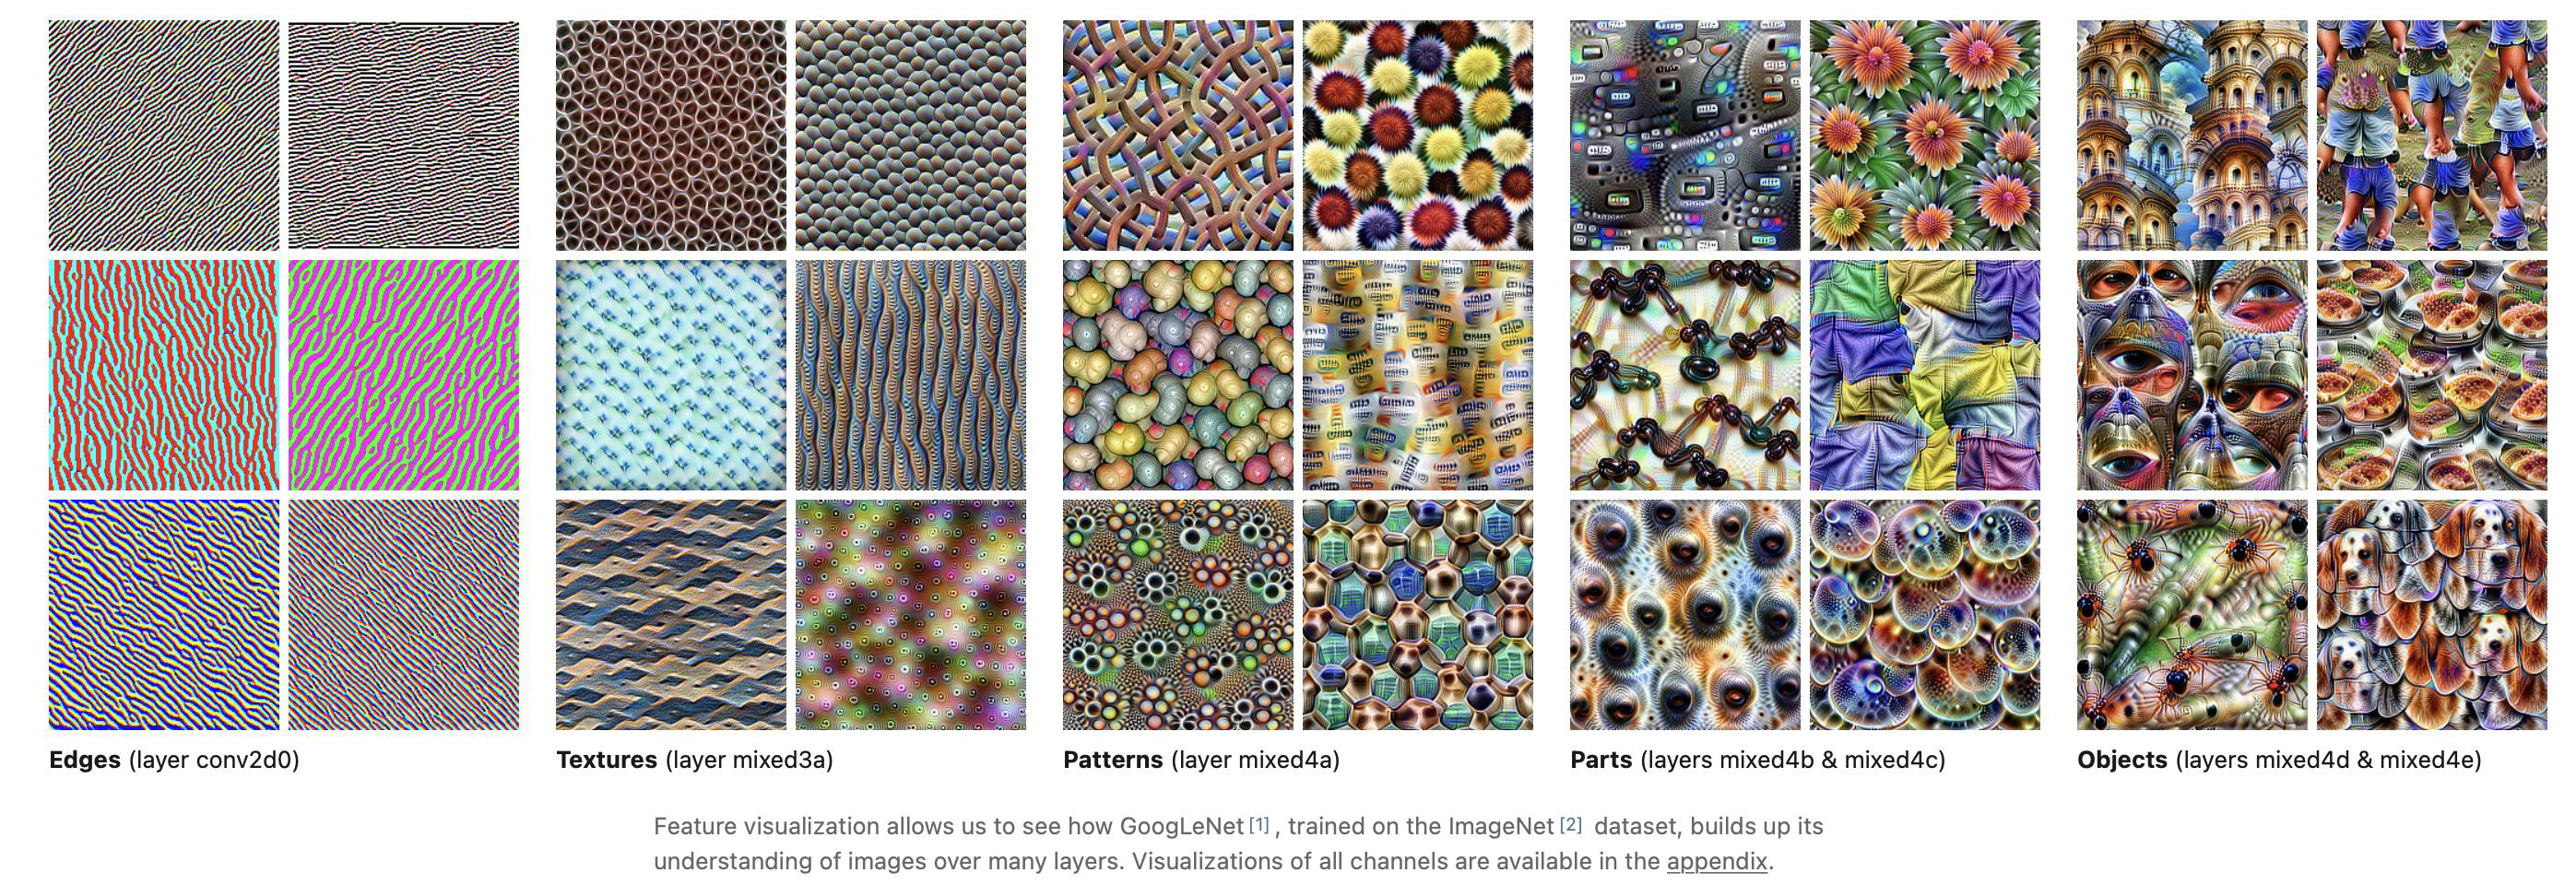
\includegraphics[width=1\linewidth]{images/week_4/visualising features 4.png}
    \caption{Progression across layers: from simple textures to recognisable object parts to full objects. This visualisation shows how CNNs build increasingly abstract representations.}
    \label{fig:features-4}
\end{figure}

\subsection{Visualisation Techniques}

\begin{quickref}[Feature Visualisation Methods]
Several techniques exist to understand what CNN features represent:

\begin{enumerate}
    \item \textbf{Neuron visualisation}: Generate an image that maximally activates a specific neuron at position $(x, y, z)$ in a layer (where $x, y$ are spatial coordinates and $z$ is the channel index). This shows what pattern that neuron ``looks for''.

    \item \textbf{Channel visualisation}: Optimise for an entire feature map/channel to see what patterns that filter detects across all spatial positions.

    \item \textbf{Layer visualisation} (DeepDream): Amplify patterns across an entire layer, creating dreamlike images that reveal what patterns the layer collectively detects.

    \item \textbf{Class visualisation}: Generate an image that maximises the probability of a specific class (e.g., ``dog''). This shows what features are most strongly associated with that class.
\end{enumerate}

All these methods typically use gradient ascent: start with noise and iteratively modify the image to increase the target activation.
\end{quickref}

\subsection{Examples of Learned Features}

The progression of learned features follows a consistent pattern across different CNN architectures:

\begin{itemize}
    \item \textbf{Edges}: First layers learn Gabor-like filters detecting vertical, horizontal, and diagonal edges at various orientations
    \item \textbf{Colours and gradients}: Simple colour blobs and smooth transitions
    \item \textbf{Textures}: Repeating patterns like grids, circles, scales, and woven structures
    \item \textbf{Patterns}: More complex recurring motifs-floral patterns, geometric structures, animal prints
    \item \textbf{Parts}: Recognisable object components-eyes, wheels, windows, petals
    \item \textbf{Objects}: Full object representations formed by combining parts-faces, animals, vehicles
\end{itemize}

\begin{quickref}[Why Visualisation Matters]
\begin{itemize}
    \item \textbf{Interpretability}: Understand what the network actually learns, not just that it works
    \item \textbf{Debugging}: Identify unexpected or biased features (e.g., a classifier detecting backgrounds rather than objects)
    \item \textbf{Trust}: Critical for safety-sensitive applications (medical imaging, autonomous driving) where we need to understand failure modes
    \item \textbf{Research}: Provides insights into representation learning and how neural networks process visual information
    \item \textbf{Education}: Makes abstract neural network concepts concrete and intuitive
\end{itemize}
\end{quickref}
